\section{Design}
\label{sec:design}
Stitch~\cite{Bowers_2023stitch} uses a corpus guided top down search approach directly, which works on the lisp-like programs expected by Stitch, but the approach naively fails in less regular languages due to correctness issues: extracted common subtrees may not, in fact, be valid in the original language.

For example, when Stitch is given a Python's abstract syntax tree (AST) represented in a lisp style, 
% (tweaked to have a lisp-like lambda format) 
some elements or expressions, like the keywords "while" and "if", or operators like "==" and ">", are treated as first-class citizens of the programming language --- extracted subtrees could contain variables that hold such values, or functions could be called with these elements as parameters, resulting in syntactically incorrect calls, 
e.g.\ \texttt{compare(1,2,==)} or assignments, e.g.\ \texttt{x = while}.
% either variable names or function names depending the lamlispifying implementation.
Broadly, this issue arises because Stitch assumes a regular lambda calculus represented in a lisp style, and a Python AST is not sufficiently regular. 
% So, it has no knowledge of what would be a valid abstraction in a language like Python. 

% is unaware of the programming language it is abstracting over, but instead 
% This can result in incorrect abstractions, like an abstraction that expects "if" or "while" as arguments and treats them as variables. Hence, 
% To better generalize Stitch and extend it to a language like Python, we identify and prune such invalid abstractions. 
\toolname{} extends Stitch to correctly extract a library from a corpus of the language \ptwo{}, a large formal subset of Python 3 developed by Siek and Chang~\cite{pythonbook} in their textbook for compiler instruction. All \ptwo{} programs are valid Python 3 programs with equivalent behavior.  The \ptwo{} language supports imperative-style programming, with scoped variable assignment, control, function calls and non-nested definitions.  The language is dynamically typed across integer, booleans, lists, and dictionaries, with support for corresponding operations and comparisons.  Output is done through the \texttt{print} keyword, and input handled via a fixed expression \texttt{eval(input())}, which takes user input, represented as an unsupported string type, and casts it to the appropriate type (e.g.\  if the user inputs \texttt{``True''}, the return value of the corresponding \texttt{eval(input())} expression will be the boolean \texttt{True} value).  The full grammar of \ptwo{} is reproduced in the appendix.
% JI: we should remove lambdas?

The architecture of our \toolname{} tool is shown in Figure ~\ref{fig:design}. As input,
\toolname{} expects in a corpus of \ptwo{} programs.  In the first step (\emph{lispify}), it coverts the \ptwo{} programs into a lisp-like format recognizable to Stitch~\cite{Bowers_2023stitch}.  Stitch then proposes a lisp-like candidate for extraction.  The candidate is subsequently subjected to a series of \emph{pruning} checks that verify that the candidate can, indeed, be converted into a valid \ptwo{} function.  These checks correspond with a variety of issues that arise from Python's lack of regularization, and we describe them in depth in the following sections.  Once the candidate is verified, we use liveness analysis to add necessary parameters and return values --- this \emph{closing} is needed to handle the scope of live-in and live-out values from the candidate.  The final step is to \emph{pythonize} by converting the candidate back to standard \ptwo{} and adjusting the corresponding call sites.

In the following subsections, we cover each step of the \toolname{} pipeline in detail.



\begin{figure*}
  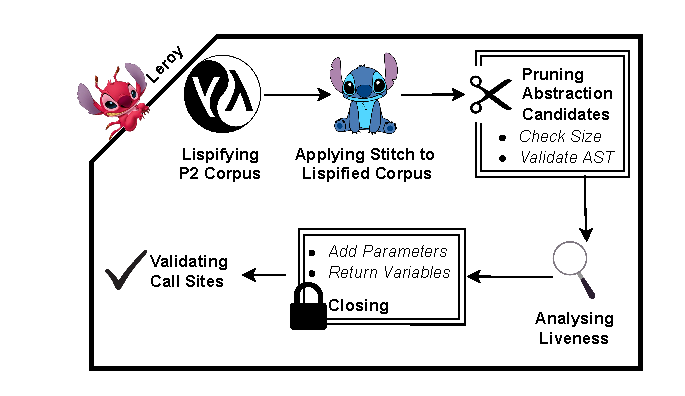
\includegraphics[width=\textwidth]{images/Design2.pdf}
  \caption{Architecture of the \toolname{} tool}
  \label{fig:design}
\end{figure*}

\todo{add the new more detailed figure}
\subsection{Problems}
\toolname extends Stitch by resolving \todo{six} main issues that arise when naively passing a lisp-like python AST to Stitch: 


\begin{enumerate}
    \item Trivial Abstractions:
    Because stitch optimizes on the abstracted function size relative to its use, it may abstract highly repeated single-line functionalities. This is \tocheck{because: such functionality is found in abundance within the code-base, and, there are no other larger abstraction candidates}. This results in functions that, for example, simply adds two numbers. \toolname eliminates such abstractions by imposing a lower constraint on abstraction size.
    \item Macro-like Abstractions: 
    Stitch treats abstracted libraries like macros\tocheck{, as it knows no better than to treat all program elements as first-class citizens}. When a functionality is abstracted, it can simply be swapped with a call. This approach impacts program correctness as it results in incomplete abstractions, like abstracting "exp + " from exp+exp. A potential abstraction $add(exp)$ would replace an addition of $1+2$ with the call $add(1) 2$. This is clearly invalid syntax.
    
    \toolname resolves this by reconstructing the AST in Python and checking its validity. 
    % To eliminate such abstractions, \toolname reconstructs the python AST from the suggested abstractions, and eliminate suggestions that fail to reconstruct a correct AST.  
    \item Invalid Parameters:
    The search method of stitch treats all tree nodes as potential "holes", or function parameters, which is incorrect in the case of python whose AST nodes are not all first-class citizens. For example, when stitch abstracts over comparative sub-trees, like "x == y" or "x!=z" it can suggest abstractions that takes three parameters, two operands and a comparison operator. A potential abstraction $f(x,op,y)$ would need to be called like: $f(x, ==, y)$ or $f(x, !=, y)$. This is clearly invalid syntax.
    
    \toolname also resolves this by reconstructing the AST in Python and checking its validity. 
    \item Incomplete return set:
    Because Stitch treats abstractions as macros, it does not consider variable scoping in abstractions, which impacts code correctness in a language like python. For example, Stitch can abstract assignments without returning the assignment targets. That is, it can suggest functions that change the value of a variable, but never returns the changed variable. In python, such assignment will create a new variable local to the abstracted (called) function instead of changing the value of the variable from the calling function. This, although syntactically correct, changes the program behaviour. \todo{To address this issue \toolname performs a liveness analysis to determine what variables are live out of the abstraction call, and returns those.}

    \item Incomplete Parameter Set:
    Some abstractions may use a variable that is not defined in the abstraction scope. This maybe because the same variable name is used in similar code-fragments across the corpus. As a result, that variable doesn't become a parameter to the abstraction.  
    To find these variables \toolname performs a liveness analysis to determine variables that aren't live into the abstraction's body. It is assumed that these variables exist in the calling scope, and they are added as parameters to the abstraction.

    \item Validating the correctness of call sites:

    Some abstraction calls may be invalid, as parameters passed to the abstraction may need to be recomputed within the abstraction's body. 
    Although we are able to find macro-like abstractions which are not valid python ASTs, these abstraction calls are still be macro-like.
    To validate the correctness of call-sites, we check that no parameter's expression is killed inside the abstraction. \toolname removes such abstraction calls.

\end{enumerate}





% \toolname performs library extraction by operating on the Abstract Syntax Tree (AST) of a subset of Python. It compiles a python AST into a lisp-like syntax that adheres to Stitch's grammar, then utilizes Stitch \cite{Bowers_2023stitch} as the library extraction engine, \toolname prunes invalid abstractions produced by Stitch to present the most useful suggestions to the developer, and compiles the output back to a python AST. Figure \ref{fig:design} illustrates the high-level design of \toolname.



\subsection{Lispifying}
To use Stitch, \toolname must first convert the \ptwo{} program into a Lisp-like representation. 
This conversion treats AST nodes as nested function calls, where each node acts as a function and its child nodes as arguments. This approach enables \toolname to unfold the AST into a single, unified function call, simplifying the abstraction process. For instance, consider an AST representing \tocheck{the addition operation $1+2$. The AST would look like a tree, with an 'add' node at the root and $1$, $2$ as it's children. Refer figure \ref{figure:LibAbsAST} for a depiction. We can also represent the tree as this function call `add(1, 2)`, where the left and right children are the first the second operands respectively.}. In Lisp-like form, this would appear as `(add 1 2)`. 

\tocheck{Additionaly, \toolname lispifies a list of statements (like a function's body) as a cascading list of function calls. As an example, consider the following three statements $x=1$, $y=1$, $print(x+1)$. \toolname encodes this as $StatementList(x=1, StatementList(y=1, StatementList(print(x+y), \epsilon)))$, where $\epsilon$ is the empty statement. This encoding draws inspiration from the `let` statement in Lisp. We do this to allow statements in the middle of a function to be abstracted. This is a crucial step in the encoding process that allows the creation of many more abstractions.
As a result, Stitch is capable of suggesting abstractions like $StatementList(x=1, StatementList(y=1, ?))$, where the $?$ is a parameter to the abstraction. In this case, the statement list $StatementList(print(x+y), \epsilon)$ would be passed as a parameter. \toolname ensures to pluck out this extra argument and place the statement back in the abstractions calling scope.}

After utilizing Stitch, \toolname converts the lisp-like syntax to a python AST which can then be unparsed to correct python code. 


\subsection{Pruning Stitch's Abstractions}
Stitch suggests many abstractions that may not port well to Python. To refine these abstractions, \toolname employs pruning strategies. Other valid abstractions are augmented with additional information, such as adding return statements, or accepting more parameters in the abstraction's signature. 

\subsubsection{Macro-Like Abstractions}
To identify and prune macro-like abstractions where the abstraction is an incomplete python code, \toolname attempts to reconstruct the abstraction into a program AST form, then checks for the correctness of the yielded AST. It verifies the completeness of the AST by ensuring all required child nodes of a parent node exist. Incomplete ASTs are indicative of macro-like structures leading them to be subsequently pruned. For example, an incomplete AST might involve a function call without required arguments, such as `(add a)` where `b` is missing. 

\subsubsection{Invalid Parameters}

Additionally, \toolname identifies cases where abstractions incorporate invalid parameters. It analyzes the abstraction’s body by converting it back into a program AST and encoding parameters as identifier nodes. By validating these nodes against the AST structure, \toolname ensures the legitimacy of parameter usage within the abstraction. For instance, in a comparison expression `(a > b)`, Stitch may produce an abstraction of the form \texttt{compare(a, comparator, b)} instead of \texttt{greater\_than(a,b)}. Such abstractions that take in invalid parameters are pruned out. 

\subsubsection{Presenting Non-trivial Abstractions}

To enhance the utility of suggested abstractions, \toolname filters out trivial cases by imposing a minimum size requirement. This criterion ensures that the extracted abstractions are sufficiently complex and meaningful to warrant inclusion. This enforces trivial functions, like simple addition or printing, are not abstracted alone despite having a high utility due to its high usage frequency. 

\subsubsection{Determining the Return Value}

\toolname complements the abstractions generated by Stitch by ensuring a coherent return value, if absent. 

To find what needs to be returned, \toolname performs a liveness analysis, to determine what variables are live out of the abstraction body. This is done by examining the target site of the abstraction. 
It is worth noting that the abstraction's parameters may themselves be live-out and need to be returned. 

If there are no live-variales out, \toolname reverts back to returning the last variable or expression in the abstraction’s body. 

Such an approach helps with functional correctness of the abstractions in the target programming language. For example, Stitch may produce an abstraction where a variable is updated, but does not return the variable at the end of the abstraction, thereby generating erroneous compressed code. 

\subsubsection{Determining Additional Parameters}:

Stitch's abstractions may assume the presence of certain variables, even if they aren't passed into the abstraction. This is because the same variable names appear in similar code-fragments across different parts of of the corpus. It is important to pass these as parameters to have a valid python function. We find variables that are \textit{not} live into the abstraction's body and add them as parameters. 

\subsubsection{Validating the correctness of call sites}
\toolname also checks the validity of each abstraction call, to ensure that the call doesn't change the code's functionality. As Stitch treats abstraction parameters like macros, there maybe parameters whose values need to be recomputed in the abstraction's body. 

This is best illustrated with an example. Consider the abstraction in figure \ref{fig:possible-invalid-function-call}. This function prints the value $param0$ in a loop that runs 5 iterations.

Stitch detects that this abstraction could be called at \ref{fig:invalid-targetsite}, by using the function call $func1(x+5)$. However, this is an invalid call as x+5 is re-computed every iteration in the loop; but the passing the value as $param0$ computes it only once at the call site. This changes the code's behaviour.

To detect such invalid call-sites, \toolname analyses the target site to determine that the expression $x+5$ is killed within it. As a result, the expression cannot be computed once, at the start of the target site; making this an invalid abstraction call.

In general, we determine if any parameter passed will be killed inside the body of the abstraction. If so, we deem such an abstractio call to be invalid.

\begin{figure}
    \begin{lstlisting}
    def func1(param0):
        for x in range(5):
            print(param0)
    \end{lstlisting}
    \caption{A valid function, which could be called erroneously}
    \label{fig:possible-invalid-function-call}
\end{figure}

\begin{figure}
    \begin{lstlisting}
    for x in range(5):
        print(x+5)
    \end{lstlisting}
    \caption{An invalid target site for func1}
    \label{fig:invalid-targetsite}
\end{figure}

\begin{figure}
\begin{lstlisting}
    -> func1(x+5) 
\end{lstlisting}
    \caption{An invalid call site to func1}
    \label{fig:invalid-callsite}
\end{figure}


\subsection{Pythonizing}
Finally, ASTs are converted back to python using the `ast.unparse` function.

% \subsection{Converting Abstractions back to the Programming Language AST}

% Finally, \toolname converts the refined suggestions from Stitch back into the Abstract Syntax Tree of the programming language. It then unparses the AST to yield the compressed code, integrating the identified abstractions seamlessly into the original program structure.
